\chapter{Ergebnisse}
In Kapitel 5 werden die Ergebnisse der durchgeführten Experimente dargelegt, welche die Effizienz und Genauigkeit von Document Understanding Transformers, insbesondere des Donut-Modells, im Vergleich zu traditionellen OCR-basierten Modellen und LayoutLMv3 evaluieren. Die Auswertung basiert auf den zuvor definierten Metriken: Accuracy, F1-Score und GPU-Stunden (GPUh), die eine umfassende Einsicht in die Leistungsfähigkeit der untersuchten Modelle unter realen Anwendungsbedingungen ermöglichen. Die im folgenden Kapitel präsentierten Ergebnisse und Beobachtungen sind, sofern nicht anders angegeben, Eigenleistung dieser Arbeit. Sie basieren auf den Experimenten, die mit den drei Modellen Donut, LayoutLMv3 und BERT im Rahmen dieser Bachelorarbeit durchgeführt wurden. Fremde Beobachtungen und Ergebnisse sind entsprechend gekennzeichnet.

Die Analyse der Ergebnisse beginnt mit einer detaillierten Bewertung der Modellperformance, fokussiert auf Accuracy und F1-Score. Diese Metriken spiegeln wider, wie präzise die Modelle relevante Informationen aus den Dokumenten extrahieren und Fehlinterpretationen minimieren. Es wird aufgezeigt, inwiefern das Donut-Modell seine Stärken gegenüber den herkömmlichen OCR-Systemen und LayoutLMv3 ausspielen konnte, insbesondere bei der Verarbeitung heterogener Datensätze aus dem Unternehmensumfeld. Des Weiteren wird der Einfluss der Datenmenge und -qualität auf die Modellperformance diskutiert, um zu verdeutlichen, wie diese Faktoren die Effizienz und Genauigkeit der Informationsgewinnung beeinflussen.

\section{Detailierte Ergebnisspräsentation}
Zunächst sollen in folgendem Abschnitt die besten Ergebnisse der Modellperformance in Bezug auf die Metriken Accuracy, F1-Score und GPUh präsentiert werden. Die Ergebnisse basieren auf den Experimenten, die mit den drei Modellen Donut, LayoutLMv3 und BERT durchgeführt wurden. Die Resultate der Modellperformance sind in Tabelle \ref{tab:best_results} zusammengefasst.
\begin{table}[h]    
\centering
    \begin{tabularx}{\textwidth}{lXXX}
      \toprule
      & \textbf{Donut} & \textbf{LayoutLMv3} & \textbf{BERT}  \\
      \midrule
      F1 Score & 80.2 & \textbf{92.1} & 91.1 \\
      \addlinespace
      Accuracy & 85.7 & \textbf{94.1} & 93.9 \\
        \addlinespace
        GPUh & 3.11 & 2.04 & \textbf{0.077} \\
      \bottomrule
    \end{tabularx}
    \caption{Beste Ergebnisse der Modellperformance (Epochen: 20, Schrittmenge: 100, Per-Device Train/Eval Batch-Size: 2, Evaluation: Alle 3 Epochen, Metrik für das beste Modell: F1, Learnrate: 3e-5)}
    \label{tab:best_results}
\end{table}
Es wird ersichtlich, dass Donut in keiner der Metriken die besten Ergebnisse erzielen konnte. LayoutLMv3 hingegen konnte sowohl den höchsten F1-Score als auch die höchste Accuracy erreichen. BERT hingegen benötigte die wenigsten GPU-Stunden, um die Dokumente zu verarbeiten. 

Vor der Interpretation der Ergebnisse ist hervorzuheben, dass die Leistung des Donut-Modells hinsichtlich der Accuracy und des F1-Scores mit Werten zwischen 80-85 \% durchaus zufriedenstellend ist und nahe an den in der Originalpublikation berichteten Ergebnissen liegt. \footcites[Vgl.][]{kim_ocr-free_2021} Da Donut v. a. auf englischen Daten trainiert wurde ist die Modellperformance auf deutschen Datensätzen etwas schlechter. Die Layouts von bspw. Rechnungen oder Lieferscheinen können sich in Deutschland von denen in den USA unterscheiden. Des weiteren ist anzumerken, dass das Finetuning mit 180, 300, 850 Trainingsdaten stattgefunden hat. Dies ist deutlich weniger als der Inhalt von \ac{CORD} oder \ac{FUNSD}. Diese Situation ist für die Studie vorteilhaft, da sie die tatsächliche Verfügbarkeit von Trainingsdaten in einem Unternehmen realistisch darstellt. Allerdings begrenzt sie auch das mögliche Leistungsspektrum von Donut. Zwar beschäftigt sich die vorliegende Bachelorarbeit mit der Frage, ob Donut den Prozess der Dokumentenverarbeitung effizienter und genauer gestalten kann, jedoch sollen die Referenzergebnisse von LayoutLMv3 und BERT nicht außer Acht gelassen werden, da diese ebenfalls Implikationen für die beteiligten Prozesse der Dokumentenverarbeitung haben. Potenziell könnte sich hier für Unternehmen eine Alternative zu Donut ergeben, die ebenfalls effizient und genau arbeitet.

Der niedrige F1-Score von 80 \% bei Donut deutet darauf hin, dass bei jeder fünften Vorhersage ein Fehler in der Extraktion einer Entität gemacht wird. Dies kann aus zwei Perspektiven gedeutet werden. Einerseits bedeutet es für die vollständige Automatisierung, dass regelmäßig händisch Fehlerkorrekturen vorgenommen werden müssen. Ein niedriger F1-Score für das Donut-Modell bedeutet, dass das Modell Schwierigkeiten hat, relevante Informationen aus Dokumenten effektiv zu identifizieren und zu extrahieren. Für Anwendungsfälle, in denen es kritisch ist, präzise und vollständige Informationen aus Dokumenten zu extrahieren, könnte ein niedriger F1-Score des Donut-Modells bedeuten, dass das Modell möglicherweise nicht die gewünschte Effektivität erreicht. Dies könnte zu einer erhöhten Nachbearbeitungszeit führen, um Fehler zu korrigieren oder fehlende Informationen manuell zu ergänzen, was den Automatisierungsgrad und die Effizienz der Dokumentenverarbeitung reduziert. Andererseits bedeutet es, dass in manuellen Arbeitsfeldern lediglich jeder fünfte Eintrag von einer Person nachbereitet werden muss. In Umfeldern, in denen noch keine Automatisierung besteht, kann Donut daher eine kostengünstige Alternative bieten, um Mitarbeiter in der Dokumentenverarbeitung zu entlasten.

Die Accuracy von rund 85 \% beim Donut-Modell bedeutet, dass ein signifikanter Anteil der vom Modell getroffenen Vorhersagen über das gesamte Spektrum möglicher Klassen (z. B. relevante Informationen, irrelevante Informationen, verschiedene Arten von Informationen etc.) falsch ist. Auch im Hinblick auf die Accuracy ist es wichtig, die Ergebnisse von Donut im Kontext der spezifischen Anforderungen und Anwendungsfälle zu interpretieren, um zu beurteilen, ob das Modell die gewünschte Genauigkeit und Zuverlässigkeit bietet. Im Falle der Implementierung von Donut in der Endanwendung würde die niedrige Accuracy bedeuten, dass das Modell eine beträchtliche Anzahl von Fehlern bei der Informationsgewinnung macht, was die händische Nachbearbeitung und Korrektur von Dokumenten erfordert. Bei solch einer hohen Anzahl an Fehlern ist jedoch fraglich, ob der Einsatz von Donut tatsächlich zu einer Effizienzsteigerung führen würde, da die manuelle Nachbearbeitung einen erheblichen Zeitaufwand erfordert und die Vorteile der Automatisierung zunichtemacht.

Auch im Hinblick auf die Effizienz (GPUh) konnte Donut nicht besser abschneiden als die Referenzmodelle. Mit 3.11 GPU-Stunden benötigt Donut mehr als das 40-fache an Rechenleistung als BERT, um die Dokumente zu verarbeiten. Dies ist ein deutlicher Hinweis darauf, dass Donut nicht nur in der Modellperformance, sondern auch in der Effizienz hinter den Referenzmodellen zurückbleibt. Die hohe Anzahl an GPU-Stunden, die Donut benötigt, um die Dokumente zu verarbeiten, bedeutet, dass das Modell sehr rechenintensiv ist und eine erhebliche Menge an Rechenressourcen in Anspruch nimmt. Es sei gesagt, dass BERT kein layoutbasiertes Modell ist und beim Training keine Bilder verarbeiten muss. Nichtsdestotrotz hat LayoutLMv3 ebenfalls eine viel höhere Effizienz als Donut. Diese Zahlen müssen jedoch im Kontext betrachtet werden. Zwar benötigt Donut mehr GPU-Stunden als die Referenzmodelle, jedoch ist die Anzahl an GPU-Stunden insgesamt sehr gering. Die Kosten für die Rechenleistung von Donut in der Rechenumgebung beliefen sich bei einem Trainingsdatensatz von 850 Dokumenten, einer Schrittmenge von 100 und 30 Epochen auf 18,36 \$. Dies ist ein sehr geringer Betrag, der in den meisten Unternehmen keine signifikante Rolle spielen sollte.

\section{Ergebnisinterpretation und Implikationen}
Die Ergebnisse der Modellperformance zeigen, dass Donut im Vergleich zu den Referenzmodellen LayoutLMv3 und BERT in den Metriken Accuracy, F1-Score und Effizienz (GPUh) nicht die besten Ergebnisse erzielen konnte. Es gilt nun zu untersuchen, welche Faktoren einen Einfluss auf die Modellperformance haben, um so die in Kapitel 3 aufgestellten Hypothesen zu überprüfen und die Forschungsfrage zu beantworten.

Der wohl entscheidendste Faktor ist die Größe und Qualität des Datensatzes. Donut wurde mit 180, 300 und 850 Trainingsdaten trainiert. Die Graphen in Abbildung \ref{fig:experiment_results} zeigen, wie sich die Datensatzgröße auf die Metriken auswirkt. Bei Donut zeigt sich im Vergleich zu seinen Konkurrenten, dass es eine viel höhere Menge an Daten braucht, um die Modellperformance so weit zu steigern, dass Donut mehr Felder richtig erkennt als nicht. Dies ist ein Hinweis darauf, dass Donut eine hohe Menge an Trainingsdaten benötigt, um seine volle Leistungsfähigkeit zu entfalten. Dies ist ein wichtiger Aspekt, der bei der Implementierung von Donut in Betracht gezogen werden sollte, da die Verfügbarkeit von Trainingsdaten in der Praxis oft begrenzt ist. 
    
Die Qualität der Trainingsdaten ist ebenfalls ein wichtiger Faktor, der die Modellperformance beeinflusst. Wie in Kapitel 3 beschrieben, wurden die Trainingsdaten in diesem Experiment von einem leistungsfähigen Extraktionstool in Azure annotiert. BERT und LayoutLMv3 wurden mit den gleichen Daten trainiert. Es wird deutlich, dass die beiden OCR-abhängigen Modelle mit viel weniger Daten gute Ergebnisse präsentieren. Im Experiment wurde deutlich, dass LayoutLMv3 und BERT einen F1-Score über 80 \% mit lediglich 180 Daten erzielen konnten, während Donut lediglich 13 \% erreichte (Vgl. dazu Abb. \ref{fig:experiment_results} und Tab. \ref{tab:donut_metrics}).Eine genauere Betrachtung im Training zeigt, dass die OCR-abhängigen Modelle viel weniger Daten brauchen, um die gewünschten Labels zu lernen. Bspw. kann LayoutLMv3 auch untrainiert Felder schon an den richtigen Positionen erkannt haben. Die Vorhersage entsprach jedoch noch nicht dem Label, gegen welches geprüft wurde. Ein Beispiel wäre, dass LayoutLMv3 auch untrainiert, ein Lieferdatum in einem Dokument erkennt, aber dieses nicht als \emph{Lieferdatum} annotiert, sondern als \emph{Delivery Date}. Das passiert, da das Modell ursprünglich auf englischen Daten trainiert wurde. Zwar wäre das Feld fachlich gesehen richtig erkannt gewesen. Jedoch würde bei der Prüfung gegen die zugrunde liegende Ground Truth das Feld als falsch gewertet werden, da es nicht spezifisch \emph{Lieferdatum} heißt. Bei den OCR-abhängigen Modellen verschwindet dieser Effekt schon bei sehr wenigen Daten. Donut hingegen benötigt jedoch mehr als 200 Trainingsdaten, um die Labels zu lernen.

\pgfplotsset{compat=1.9}

\begin{figure}
\centering
% F1 Score
\begin{minipage}{.32\textwidth}
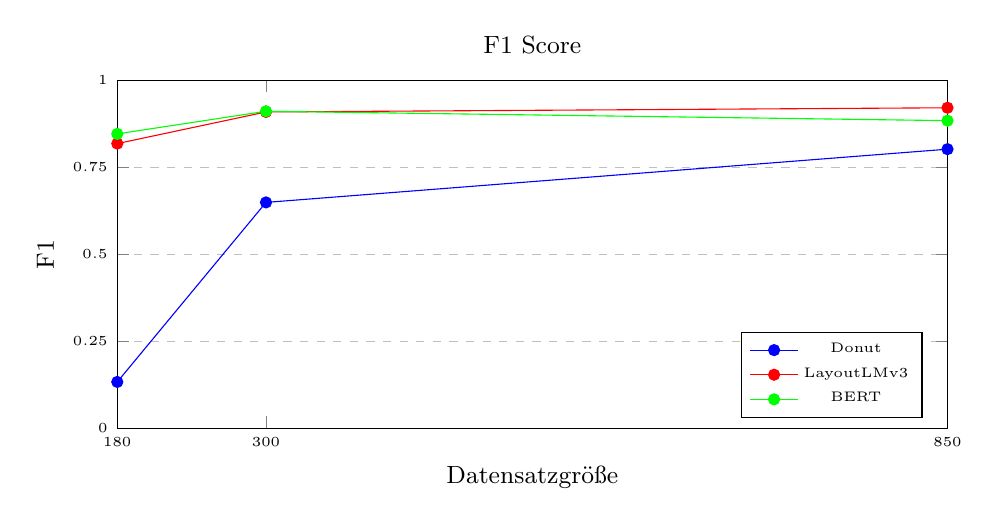
\begin{tikzpicture}
\begin{axis}[
    title={F1 Score},
    xlabel={Datensatzgröße},
    ylabel={F1},
    xmin=180, xmax=850,
    ymin=0, ymax=1,
    xtick={180,300,850},
    ytick={0,0.25,0.5,0.75,1},
    tick label style={font=\tiny},
    label style={font=\small},
    title style={font=\small},
    legend style={font=\tiny},
    legend pos=south east,
    ymajorgrids=true,
    grid style=dashed,
    width=\linewidth, height=6cm,
]

\addplot[color=blue,mark=*,] coordinates {(180,0.133)(300,0.649)(850,0.802)};
\addlegendentry{Donut}

\addplot[color=red,mark=*,] coordinates {(180,0.818)(300,0.909)(850,0.921)};
\addlegendentry{LayoutLMv3}

\addplot[color=green,mark=*,] coordinates {(180,0.846)(300,0.911)(850,0.884)};
\addlegendentry{BERT}

\end{axis}
\end{tikzpicture}
\end{minipage}%
%
% Accuracy
\begin{minipage}{.32\textwidth}
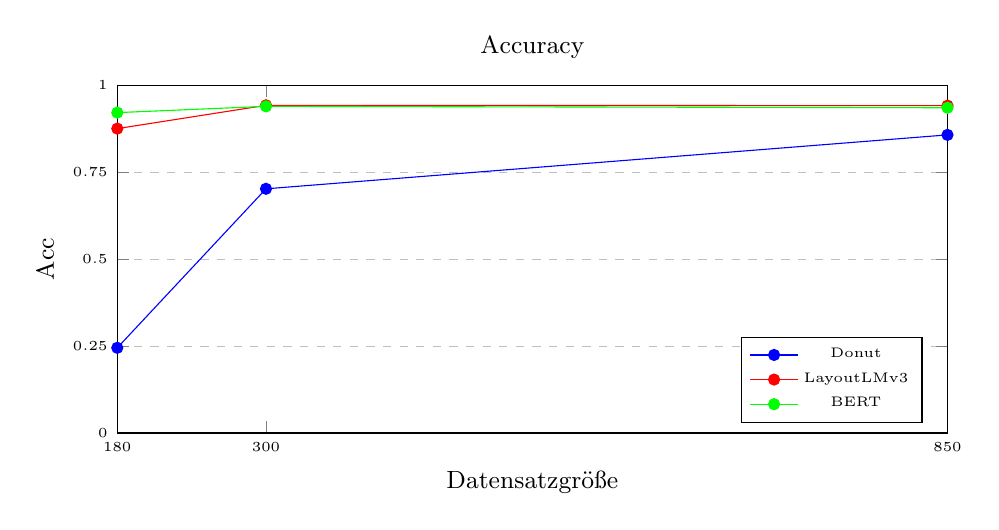
\begin{tikzpicture}
\begin{axis}[
    title={Accuracy},
    xlabel={Datensatzgröße},
    ylabel={Acc},
    xmin=180, xmax=850,
    ymin=0, ymax=1,
    xtick={180,300,850},
    ytick={0,0.25,0.5,0.75,1},
    tick label style={font=\tiny},
    label style={font=\small},
    title style={font=\small},
    legend style={font=\tiny},
    legend pos=south east,
    ymajorgrids=true,
    grid style=dashed,
    width=\linewidth, height=6cm,
]

\addplot[color=blue,mark=*,] coordinates {(180,0.245)(300,0.702)(850,0.857)};
\addlegendentry{Donut}

\addplot[color=red,mark=*,] coordinates {(180,0.875)(300,0.942)(850,0.941)};
\addlegendentry{LayoutLMv3}

\addplot[color=green,mark=*,] coordinates {(180,0.921)(300,0.939)(850,0.935)};
\addlegendentry{BERT}

\end{axis}
\end{tikzpicture}
\end{minipage}%
%
% GPU Stunden
\begin{minipage}{.32\textwidth}
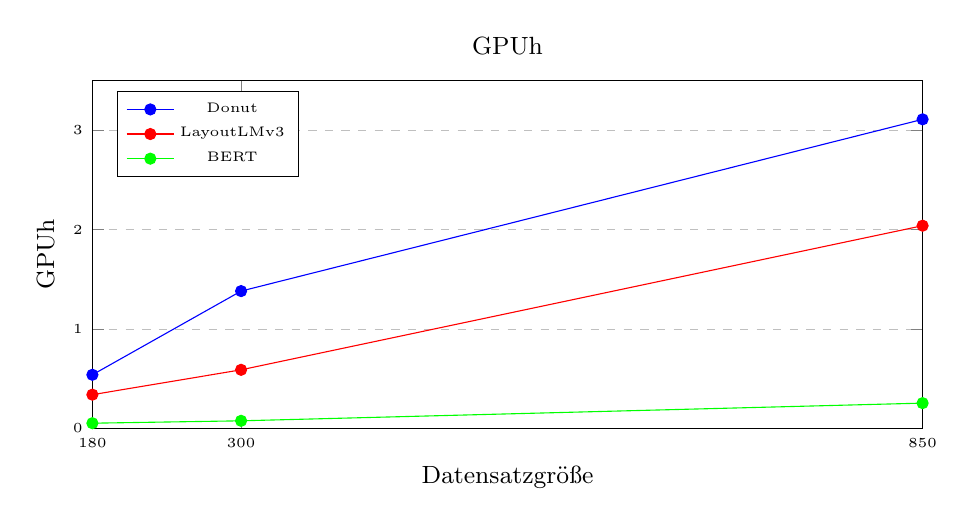
\begin{tikzpicture}
\begin{axis}[
    title={GPUh},
    xlabel={Datensatzgröße},
    ylabel={GPUh},
    xmin=180, xmax=850,
    ymin=0, ymax=3.5,
    xtick={180,300,850},
    ytick={0,1,2,3},
    tick label style={font=\tiny},
    label style={font=\small},
    title style={font=\small},
    legend style={font=\tiny},
    legend pos=north west,
    ymajorgrids=true,
    grid style=dashed,
    width=\linewidth, height=6cm,
]

\addplot[color=blue,mark=*,] coordinates {(180,0.54)(300,1.382)(850,3.11)};
\addlegendentry{Donut}

\addplot[color=red,mark=*,] coordinates {(180,0.34)(300,0.59)(850,2.04)};
\addlegendentry{LayoutLMv3}

\addplot[color=green,mark=*,] coordinates {(180,0.053)(300,0.077)(850,0.255)};
\addlegendentry{BERT}

\end{axis}
\end{tikzpicture}
\end{minipage}
\caption{Vergleich der Modellmetriken F1 Score, Accuracy und GPU Stunden (GPUh) über verschiedene Datensatzgrößen.}
\label{fig:experiment_results}
\end{figure}


\newcolumntype{Y}{>{\centering\arraybackslash}X}

\begin{table}
\centering
\begin{tabularx}{\textwidth}{@{}lYYY@{}}
\toprule
& \textbf{Donut} & \textbf{LayoutLMv3/LMv3} & \textbf{BERT} \\
\midrule
\multicolumn{4}{c}{\textbf{180 Dataset} (126 Train, 27 Test, 27 Val)} \\
\midrule
F1         & 0.133 & 0.818 & 0.846 \\
Accuracy   & 0.245 & 0.875 & 0.921 \\
GPUh       & 0.54  & 0.34  & 0.053 \\
\midrule
\multicolumn{4}{c}{\textbf{300 Dataset} (240 Train, 30 Test, 30 Val)} \\
\midrule
F1         & 0.649 & 0.909 & 0.911 \\
Accuracy   & 0.702 & 0.942 & 0.939 \\
GPUh       & 1.382 & 0.59  & 0.077 \\
\midrule
\multicolumn{4}{c}{\textbf{850 Dataset} (730 Train, 40 Test, 80 Val)} \\
\midrule
F1         & 0.802 & 0.921 & 0.884 \\
Accuracy   & 0.857 & 0.941 & 0.935 \\
GPUh       & 3.11  & 2.04  & 0.255 \\
\bottomrule
\end{tabularx}
\caption{Vergleich von Modellen über verschiedene Datensätze}
\label{tab:donut_metrics}
\end{table}

Auffällig sind die sehr guten Ergebnisse von BERT. Gegenüber der bestehenden Forschung in der Literatur hat BERT in diesem Experiment mit einer sehr guten Performance überzeugt. \footcites[Vgl. dazu ausführlich][]{kim_ocr-free_2021}[][]{huang_layoutlmv3_2022} Da die Ergebnisse stark von denen in der bisherigen Literatur abweichen, müssen diese besonders kritisch betrachtet werden. BERT verfügt über keine Möglichkeit, Layoutinformationen zu verarbeiten. Es ist daher überraschend, dass BERT so gute Ergebnisse erzielt hat. Zunächst ist es wichtig zu verstehen, welche Informationen BERT beim Training als Input erhält. BERT erhält als Input die Texte der Dokumente. Der Datensatz hält zu jedem Token ein Label fest. Dies kann an folgendem Beispiel nachvollzogen werden: 

Eine Liste aus Tokens [Technik, GmbH, 13, 12, 2022] würde bspw. das Label [CompanyName, CompanyName, DateDay, DateMonth, DateYear] erhalten. BERT lernt also die Labels anhand der Tokens. 

Es ist daher nicht verwunderlich, dass BERT so gute Ergebnisse erzielt hat. BERT hat die Labels der Tokens gelernt und kann daher sehr gut die Labels neuen Texten zuordnen. Ein entscheidender Schwachpunkt ist jedoch, dass BERT vollständig vom Inputtext in der Inferenz abhängig ist. Eine schwache vorgelagerte OCR kann die Ergebnisse daher stark beeinflussen. 

Der Einfluss der OCR zeigt sich vor allem im Vergleich bei LayoutLMv3 zwischen Finetuning und Inferenz. Im Finetuning wurden Daten durch die vergleichsweise sehr genaue Microsoft Read OCR aufbereitet. In der Inferenz hingegen wurden die Daten durch Tesseract für die Verarbeitung vorbereitet. Abbildung \ref{fig:ocr_results} zeigt die Unterschiede in der Extraktion der beiden OCR-Systeme. Es wird deutlich, dass Microsoft Read OCR sehr viel genauere Ergebnisse liefert als Tesseract. Dies zeigt sich auch in den Ergebnissen von LayoutLMv3. Während LayoutLMv3 im Finetuning sehr gute Ergebnisse liefert, sind die Ergebnisse in der Inferenz deutlich schlechter. Das Selbe trifft für BERT zu. In diesem Experiment wurden mehrere genaue Analysen einzelner Rechnungen durchgeführt. Folgende Probleme entstanden im Beispiel von Abbildung \ref{fig:ocr_results} bei der Verwendung von Tesseract:
\begin{itemize}
    \item Nur die ersten beiden Teile der IBAN wurden erkannt.
    \item Ein nicht vorhandenes Bezahlt-Feld wurde fünf Mal erkannt.
    \item Der Mehrwertsteuersatz wurde sechs Mal erkannt.
    \item Ein nicht vorhandener Rabatt in Prozent wurde erkannt.
    \item Die nicht vorhandene Umsatzsteuer-ID wurde nicht erkannt.
    \item Das nicht vorhandene Land des Verkäufers wurde erkannt.
    \item Das Fälligkeitsdatum wurde zwei Mal erkannt.
    \item Alle weiteren Felder, die in Abbildung \ref{fig:ocr_results} links zu sehen sind, aber nicht rechts, wurden nicht erkannt.
\end{itemize}

\begin{figure}[]
    \centering
    % Include the first image with specific dimensions
    \includegraphics[width=0.45\textwidth,height=0.4\textheight,keepaspectratio=false]{graphics/ms_read.png}
    \hfill % This adds space between the images
    \hfill
    % Include the third image with specific dimensions
    \includegraphics[width=0.45\textwidth,height=0.4\textheight,keepaspectratio=false]{graphics/tesseract.png}
    \caption{Links: Extraktion durch Microsoft Read OCR. Rechts: Extraktion durch Tesseract.}
    \label{fig:ocr_results}
\end{figure}

Des Weiteren müssen die niedrigen GPUh ebenso unter dem Umstand der Abwesenheit von jeglichen layoutbasierten Informationen betrachtet werden. BERT benötigt keine Bilder und kann daher sehr schnell arbeiten.

Tabelle \ref{tab:donut_metrics} zeigt die Metriken des Donut-Modells über verschiedene Datensatzgrößen. Es wird deutlich, dass die Modellperformance mit steigender Datensatzgröße zunimmt. Donut benötigt eine hohe Menge an Trainingsdaten, um die Labels zu lernen. Dies ist ein wichtiger Aspekt, der bei der Implementierung von Donut in Betracht gezogen werden sollte, da die Verfügbarkeit von Trainingsdaten in der Praxis oft begrenzt ist. Aus den Ergebnissen wird ebenfalls deutlich, dass die benötigten GPUh für das Modell mit steigender Datensatzgröße zunehmen. Auf der anderen Seite nimmt die Änderungsrate von F1-Score und Accuracy mit steigender Datensatzgröße ab. Dies bedeutet, dass das Modell mit steigender Datensatzgröße nicht mehr so stark an Performance gewinnt, wie es bei kleineren Datensätzen der Fall ist. Für Unternehmen ist es daher wichtig, die Kosten und den Nutzen von zusätzlichen Trainingsdaten abzuwägen, um eine effiziente und effektive Implementierung von Donut zu gewährleisten. Sicherlich gibt es hierfür auch andere Ansätze, wie bspw. das Training auf synthetischen Daten. Dieser Ansatz wurde jedoch in dieser Arbeit nicht weiter verfolgt. Für jedes Unternehmen gibt es wahrscheinlich eine optimale Datengröße, die die Kosten und den Nutzen von zusätzlichen Trainingsdaten ausbalanciert. Dies hängt jedoch davon ab, wie wichtig die Genauigkeit und Effizienz der Dokumentenverarbeitung für das Unternehmen sind. Daher kann diese Frage in dieser Arbeit nicht weiter verfolgt werden.

Die Ergebnisse zeigen, dass Donut in der Modellperformance hinter den Referenzmodellen zurückbleibt. Die Schwäche von Donut im Vergleich zu den Referenzmodellen ist der hohe Datenbedarf. Die Stärke von BERT liegt v. a. in seiner Leichtgewichtigkeit. Demgegenüber steht die Schwäche, dass BERT keine Layoutinformationen verarbeiten kann. LayoutLMv3 hingegen ist sehr gut in der Lage, Layoutinformationen zu verarbeiten. Von daher sind die sehr guten Ergebnisse von BERT dadurch zu erklären, dass die Daten von der ohnehin sehr performanten Microsoft Read OCR annotiert und verarbeitet wurden. 

\pgfplotsset{width=10cm,compat=1.9}

\begin{figure}[h]
    \centering
    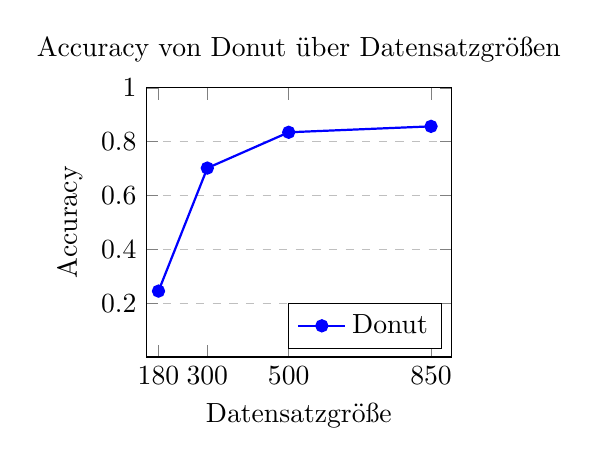
\begin{tikzpicture}
    \begin{axis}[
        title={Accuracy von Donut über Datensatzgrößen},
        xlabel={Datensatzgröße},
        ylabel={Accuracy},
        width=0.45\linewidth,
        height=5cm,
        xmin=150, xmax=900,
        ymin=0, ymax=1,
        xtick={180,300,500,850},
        ytick={0.2, 0.4, 0.6, 0.8, 1.0},
        legend pos=south east,
        ymajorgrids=true,
        grid style=dashed,
    ]
    
    \addplot[
        color=blue,
        mark=*, % Markierungsstil
        thick, % Linienstärke
        ]
        coordinates {
        (180,0.245)(300,0.702)(500,0.835)(850,0.857)
        };
        \addlegendentry{Donut}
    
    \end{axis}
    \end{tikzpicture}
     % Platz für das zweite Diagramm
    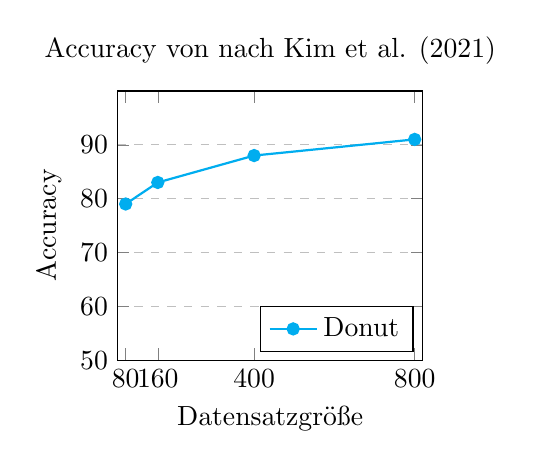
\begin{tikzpicture}
    \begin{axis}[
        title={Accuracy von nach Kim et al. (2021)},
        xlabel={Datensatzgröße},
        ylabel={Accuracy},
        width=0.45\linewidth,
        height=5cm,
        xmin=60, xmax=820,
        ymin=50, ymax=100,
        xtick={80, 160, 400,800},
        ytick={50, 60, 70, 80, 90},
        legend pos=south east,
        ymajorgrids=true,
        grid style=dashed,
    ]
    
    \addplot[
        color=cyan,
        mark=*, % Markierungsstil
        thick, % Linienstärke
        ]
        coordinates {
        (80,79)(160,83)(400,88)(800,91)
        };
        \addlegendentry{Donut}
    
    \end{axis}
    \end{tikzpicture}
    \caption{Links: Accuracy von Donut über verschiedene Datensatzgrößen. Rechts: Accuracy nach Kim et. al. \footcites[Entnommen aus][S. 13]{kim_ocr-free_2021}}
    \label{fig:accuracy_comparison_to_kim}
    \end{figure}

\begin{figure}[h]
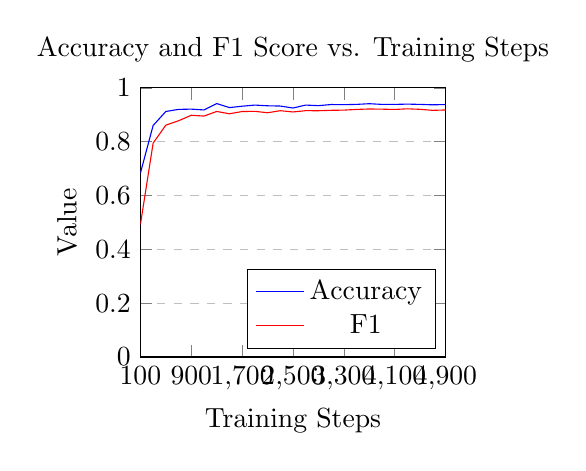
\begin{tikzpicture}
\begin{axis}[
    title={Accuracy and F1 Score vs. Training Steps},
    xlabel={Training Steps},
    ylabel={Value},
    width=0.45\linewidth, % Adjust the width to fit the line width
    height=5cm, % You can adjust the height as needed
    xmin=100, xmax=4900,
    ymin=0, ymax=1,
    xtick={100,900,1700,2500,3300,4100,4900},
    ytick={0,0.2,0.4,0.6,0.8,1.0},
    legend pos=south east,
    ymajorgrids=true,
    grid style=dashed,
]

\addplot[
    color=blue,
    mark=,
    ]
    coordinates {
    (100,0.683342)(300,0.860237)(500,0.912326)(700,0.920062)(900,0.921093)(1100,0.917999)(1300,0.941723)(1500,0.926766)(1700,0.931924)(1900,0.936050)(2100,0.933471)(2300,0.932439)(2500,0.925219)(2700,0.936050)(2900,0.933987)(3100,0.938112)(3300,0.937597)(3500,0.938628)(3700,0.941207)(3900,0.938628)(4100,0.938628)(4300,0.939660)(4500,0.938628)(4700,0.937081)(4900,0.938112)
    };
    \addlegendentry{Accuracy}

\addplot[
    color=red,
    mark=,
    ]
    coordinates {
    (100,0.492408)(300,0.794808)(500,0.861508)(700,0.877810)(900,0.898239)(1100,0.895201)(1300,0.912384)(1500,0.903827)(1700,0.912109)(1900,0.912831)(2100,0.907579)(2300,0.915238)(2500,0.910513)(2700,0.915321)(2900,0.915122)(3100,0.916626)(3300,0.917359)(3500,0.919922)(3700,0.921578)(3900,0.920898)(4100,0.919844)(4300,0.922249)(4500,0.920293)(4700,0.916545)(4900,0.917969)
    };
    \addlegendentry{F1}

\end{axis}
\end{tikzpicture}%
\hspace{1cm} % Space between the two plots
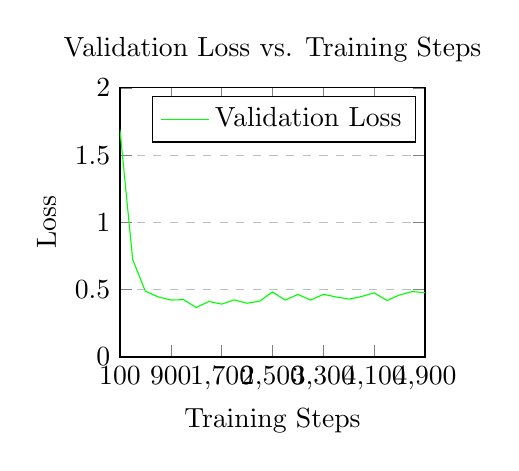
\begin{tikzpicture}
\begin{axis}[
    title={Validation Loss vs. Training Steps},
    xlabel={Training Steps},
    ylabel={Loss},
    width=0.45\linewidth, % Adjust the width to fit the line width
    height=5cm, % You can adjust the height as needed
    xmin=100, xmax=4900,
    ymin=0, ymax=2,
    xtick={100,900,1700,2500,3300,4100,4900},
    ytick={0,0.5,1.0,1.5,2.0},
    legend pos=north east,
    ymajorgrids=true,
    grid style=dashed,
]

\addplot[
    color=green,
    mark=,
    ]
    coordinates {
    (100,1.688588)(300,0.725274)(500,0.489344)(700,0.446944)(900,0.423677)(1100,0.426347)(1300,0.368085)(1500,0.413032)(1700,0.393213)(1900,0.424923)(2100,0.399802)(2300,0.415617)(2500,0.483545)(2700,0.423475)(2900,0.465307)(3100,0.423118)(3300,0.466113)(3500,0.446490)(3700,0.430447)(3900,0.449491)(4100,0.477200)(4300,0.420380)(4500,0.461550)(4700,0.486353)(4900,0.478395)
    };
    \addlegendentry{Validation Loss}

\end{axis}
\end{tikzpicture}
\caption{Abflachende Änderungsrate von F1-Score und Accuracy mit steigender Datensatzgröße bei LayoutLMv3}
\label{fig:flattening}
\end{figure}

Des weiteren stehen einige Ergebnisse im Widerspruch zur bisherigen Literatur. \footcites[Vgl.][S. 13]{kim_ocr-free_2021} Für LayoutLMv3 sowie BERT liefert die Microsoft Read OCR im Experiment dieser Arbeit hervorragende Ergebnisse. Was jedoch hinsichtlich der bisherigen Ergebnisse bestätigt werden konnte, ist die abflachende Änderungsrate von F1-Score und Accuracy mit steigender Datensatzgröße. Zwar sind die Ergebnisse beim Finetuning unter CORD um rund 5 \% besser als in dieser Arbeit, jedoch ist der Trend der abflachenden Änderungsrate der Metriken mit steigender Datensatzgröße bestätigt. Dieser Sachverhalt wird in Abb. \ref{fig:accuracy_comparison_to_kim} deutlich.

Eine weitere Beobachtung konnte bei genauerer Betrachtung der Inferenzergebnisse von Donut gemacht werden. Abbildung \ref{fig:donut_inference} zeigt auf der linken Seite die Rechnung, aus welcher in der Inferenz die Informationen extrahiert wurden. Auf der rechten Seite ist das Inferenzergebnis von Donut als JSON zu sehen. Für einen Menschen scheint die Rechnung sehr einfach interpretierbar zu sein. Der intuitive Schluss wäre, dass Donut in diesem Dokument eine hohe Genauigkeit erzielt, da viele Entitäten sogar entsprechend beschriftet sind. Allerdings zeigt sich, dass Donut in der Inferenz viele Fehler gemacht hat. Das Rechnungsdatum wurde zwar erkannt, jedoch ebenfalls fälschlicherweise als Rechnungsnummer. Das Rechnungsdatum und das Fälligkeitsdatum sind vertauscht. Eine naheliegende Vermutung ist, dass es sich beim Layout dieser Rechnung um ein im Datensatz kaum vertretenes Layout handelt. Donut hat daher Schwierigkeiten, die Informationen korrekt zu extrahieren. Zwar ist der Datensatz sehr heterogen in Bezug auf die Layouts, jedoch ist es möglich, dass Donut Schwierigkeiten hat, die Informationen aus diesem spezifischen Layout zu extrahieren. Wenn Donut mit Layouts konfronitert wird, die es nicht oder kaum kennt, kann es zu Fehlern in der Extraktion kommen. Dies ist ein wichtiger Aspekt, der bei der Implementierung von Donut in Betracht gezogen werden sollte. Es ist wichtig, dass Donut mit einer Vielzahl von Layouts trainiert wird, um die Genauigkeit und Zuverlässigkeit der Dokumentenverarbeitung zu gewährleisten. Wichtig ist anzumerken, dass dieses Beispiel nicht repräsentativ für die Inferenzergebnisse von Donut ist. Die meisten Inferenzergebnisse waren sehr gut und entsprachen den Labels. Dieses Beispiel zeigt jedoch, dass Donut Schwierigkeiten haben kann, Informationen aus spezifischen Layouts zu extrahieren.

\begin{figure}[]
    \centering
    \begin{minipage}{0.45\textwidth}
        \centering
        \includegraphics[width=\linewidth]{graphics/menti-invoice.jpeg} % Pfad zur Rechnungsgrafik
    \end{minipage}\hfill
    \begin{minipage}{0.45\textwidth}
        \centering
        \includegraphics[width=\linewidth]{graphics/menti-json.png} % Pfad zur Donut-Inferenzgrafik
    \end{minipage}
    \caption{Gegenüberstellung von Rechnung und Inferenzergebnis von Donut}
    \label{fig:donut_inference}
\end{figure}

Unter anbetracht der in diesem Kapitel präsentierten Daten können zwei der Hypothesen verifiziert und eine falsifiziert werden:
\begin{itemize}
    \item \textbf{Hypothese 1:} Eine höhere Menge an Daten verbessert die Performance der Modelle, wobei
    eine abflachende oder sogar abfallende Wirkung bei Overfitting zu beobachten ist. Die Hypothese hat sich bestätigt. Es ist anzumerken, dass Overfitting nicht durch die Datenmenge selbst erreicht werden konnte, sondern lediglich durch Hyperparameter-Tuning. Spezifisch ist Overfitting bei allen Modellen aufgetreten, wenn die Anzahl an Epochen im Training 30 überschritten hat.
    \item \textbf{Hypothese 2:} Bei heterogenen Daten erzielt Donut bessere Ergebnisse als LayoutLMv3 und BERT. Die Hypothese ist falsifiziert. Donut hat über das Experiment hinweg schlechtere Ergebnisse erzielt als LayoutLMv3 und BERT.
    \item \textbf{Hypothese 3:} Die Qualität der vorgelagerten OCR beeinflusst die Ergebnisse von LayoutLMv3 und BERT signifikant. Die Hypothese hat sich durch die detaillierte Analyse der Inferenzergebnisse bestätigt. Die Inferenzergebnisse von LayoutLMv3 und BERT waren deutlich schlechter als die Finetuning-Ergebnisse. Dies ist auf die Verwendung von Tesseract als OCR-System zurückzuführen.
\end{itemize}

\section{Tiefere Analysen}
Die bisherigen Ergebnisse und Analysen waren sehr objektiv und bezogen sich v. a. auf die Leistungsfähigkeit der Modelle selbst. In diesen Analysen werden jedoch Faktoren außer acht gelassen, die ebenfalls eine wichtige Rolle bei der Implementierung von Modellen in Unternehmen spielen. Dieser Abschnitt betrachtet all die Faktoren, die eine signifikante Rolle spielen, bis es zu einem ersten Training kommt.

Da diese Arbeit die Anwendung von Donut im Unternehmensumfeld betrachtet, ist es wichtig, die Komplexität und Fehleranfälligkeit des Modells bei der Implementierung zu betrachten. Wie zuvor erwähnt sind die Kosten für das Training für die meisten Unternehmen nicht wirklich relevant. Die Kosten für die Rechenleistung beliefen sich bei einem Trainingsdatensatz von 850 Dokumenten, einer Schrittmenge von 100 und 30 Epochen auf 18,36 \$. Die viel größere Kostenstelle macht die Implementierung aus. Bei einem angenommenen Jahresgehalt von 55600 € pro Jahr betragen die Kosten für einen Mitarbeitenden der Entwicklung rund 29 € pro Stunde. Die Implementierung von Donut in einem Unternehmen würde jedoch nicht nur die Entwicklungskosten beinhalten. Daher ist es wichtig zu betrachten, welche Kosten bei der Implementierung von Donut in einem Unternehmen anfallen würden. Die folgend aufgeführten Erkenntnisse können nur qualitativ beschrieben werden, da eine quantitative Analyse den Rahmen dieser Arbeit sprengen würde. Die Erkenntnisse stammen aus den Erfahrungen des Entwicklungsprozesses der in Kapitel 4 beschriebenen Verarbeitungspipeline.

Die Entwicklung der Pipeline zeigte, dass Donut sehr fehleranfällig in Bezug auf seine Trainingsdaten ist. Im Annotationsprozess kann es manchmal vorkommen, dass eine JSON-Datei leere Felder enthält. Datensätze, welche mit der \textbf(datasets)-Bibliothek aufbereitet wurden, können problemlos mit leeren Feldern umgehen. Da es für das Label kein Token gibt, wird das fehlerhafte Feld in der Verarbeitung übersprungen. Wenn die Daten mit dem DonutDataset aufbereitet werden, führt bereits ein fehlerhafter Eintrag dazu, dass das gesamte Training abgebrochen wird. Dies ist ein sehr kritischer Punkt, da es sehr schwierig ist, Fehler in den Trainingsdaten zu finden. Bei kleineren Mengen ist dies noch möglich. Jedoch wird bei Mengen, die 100 Daten überschreiten, die händische Korrektur schwierig. Einen Vorteil, den das DonutDataset in diesem Zusammenhang bietet, ist dass die Daten sich bis vor die Verarbeitung vom jeweiligen Processor (s. Abb. \ref{fig:pipeline}) in einem Format von JSON und Bildern befinden. Dies ermöglicht eine für den Menschen einfache Überprüfung der Daten. Im Gegensatz dazu befinden sich die Daten bei der Verwendung der datasets-Bibliothek in einem Format, welches für den Menschen nicht ohne weiteres lesbar ist. Es ist sehr aufwendig, diese in ein lesbares Format zu bringen. Das Zurückführen von Fehlern auf bestimmte Daten sehr schwierig. Jedoch kam es nie zu einem Abbruch des Trainingsprozesses bei LayoutLMv3 oder BERT. Jedoch kam es sehr häufig zu einem Abbruch beim Training von Donut. Dies ist ein entscheidender Schwachpunkt, der bei der Implementierung von Donut in einem Unternehmen berücksichtigt werden sollte.

Die Trainingszeiten sind ebenfalls ein wichtiger Faktor in der Kostenrechnung. Abseits der bereits präsentierten GPUh soll eine kurze Betrachtung erfolgen, wie sich die Trainingszeiten zusammensetzen. Bei Donut ist aufgefallen, dass über 40 \% der Trainingszeit auf die Validierung entfallen. Während es bei LayoutLMv3 und BERT für 80 Validierungsdaten nur wenige Sekunden dauert, bis die Validierung in einer Epoche abgeschlossen ist, dauert es bei Donut mehrere Minuten. Wie dieser Zeitunterschied zustande kommt, konnte nicht weiter untersucht werden. Es wurden mehrere Argumentationen basierend auf der Architektur von Donut vorgeschlagen. Keine Erklärung kann jedoch als gesichert angesehen werden. Daher überlässt es diese Bachelorarbeit künftigen Arbeiten eine Erklärung für diesen Sachverhalt zu finden. Dies hat nicht nur zur Folge, dass die benötigten GPUh steigen, sondern auch, dass beim Testen des Finetunings mehr Zeit benötigt wird. 

Zuletzt gilt es zu betrachten, wie Modelle auf unterschiedliche Hyperparameter reagieren. Die initiale Hyperparameterkonfiguration sieht wie folgt aus:
\begin{itemize}
    \item \textbf{Learning Rate:} 3e-5 - Bestimmt, wie schnell oder langsam das Modell während des Trainings lernt.
    \item \textbf{Per-device Train Batch Size:} 2 - Bestimmt, wie viele Datenpunkte das Modell auf einmal verarbeitet.
    \item \textbf{Per-device Eval Batch Size:} 2
    \item \textbf{Epochs:} 30 - Bestimmt, wie oft das Modell über den gesamten Datensatz trainiert wird.
    \item \textbf{Val-check-interval:} 0.1 - Bestimmt, wie häufig das Modell während einer Epoche validiert wird (in diesem Fall 40 \% der Trainingsschritte pro Epoche)
    \item \textbf{Check-val-every-n-epoch:} 3 - Das Modell wird alle drei Epochen auf Validierungsdaten überprüft. 
    \item \textbf{Warmup Steps:} 81 - Anzahl der Schritte zu Beginn des Trainings, in denen die Lernrate schrittweise erhöht wird. 
\end{itemize}
Die Hyperparameterkonfiguration wurde für alle Modelle gleich gewählt. Es ist jedoch zu erwähnen, dass die Hyperparameterkonfiguration für jedes Modell individuell optimiert werden sollte. Die Hyperparameterkonfiguration hat einen signifikanten Einfluss auf die Modellperformance und die Trainingszeit. Die Analyse der Trainings ergab, dass die Hyperparameterkonfiguration für das Training aller Modelle nicht optimal ist. Zunächst wird in Abb. \ref{fig:flattening} deutlich, dass ab einer gewissen Anzahl an Trainingsschritten die Änderungsrate von F1-Score abflacht. In diesem Beispiel schwankte der F1-Score mit 0.5 \% um den Wert von 93.6 \%. Die folgenden Trainingsschritte schwanken anschließend um einen bestimmten Wert. Nachdem dieser Schritt erreicht ist, wird das Modell unnötig weitertrainiert, da keine Verbesserung mehr stattfindet. Eine Senkung der Epochen auf 20 konnte hier für alle Modelle ein Drittel der Trainingszeit einsparen. Die Validierung pro Epoche konnte auf 40 \% reduziert werden. Es entstand kein nennenswerter Verlust von F1. Die Lernrate war mit 3e-5 für alle Modelle zu niedrig. Eine Erhöhung auf 1e-5 konnte in viel kürzerer Zeit die zuvor präsentierten Ergebnisse erreichen. Die Instabilität stieg nicht nennenswert an. Eine Erhöhung der Batch Size hatte keinen nennenswerten Effekt auf die Trainingszeit. Schlussendlich führte eine Reduktion der Anzahl an Validierungen zu einer Verschlechterung des F1-Scores von bis zu 7 \% bei Donut und einer Verschlechterung der Accuracy von rund 5 \%. Eine Erhöhung der Validierungen führte zu keiner Verbesserung der Metriken, jedoch stieg die Trainingszeit v. a. für Donut unter Anbetracht der verlängerten Validierungszeit erheblich. Unter Beachtung dieser Ergebnisse wurde für das Erreichen der besten Ergebnisse (s. Tab \ref{tab:best_results}) folgende Konfiguration verwendet:
\begin{itemize}
    \item \textbf{Learning Rate:} 3e-5
    \item \textbf{Per-device Train Batch Size:} 2
    \item \textbf{Per-device Eval Batch Size:} 2
    \item \textbf{Epochs:} 20
    \item \textbf{Val-check-interval:} 0.4
    \item \textbf{Check-val-every-n-epoch:} 3
    \item \textbf{Warmup Steps:} 81
\end{itemize}

\section{Zusammenfassende Bewertung}
In Kapitel 5 wurden die Ergebnisse der empirischen Untersuchung präsentiert, die die Leistungsfähigkeit des Donut-Modells im Vergleich zu den etablierten OCR-basierten Modellen LayoutLMv3 und BERT unter realen Anwendungsbedingungen evaluiert haben. Dabei standen die Metriken Accuracy, F1-Score und GPU-Stunden im Fokus, um ein umfassendes Bild der Modellperformance zu liefern.

Die Analyse der Ergebnisse zeigt, dass Donut in allen drei betrachteten Metriken hinter seinen Konkurrenten zurückbleibt. Insbesondere bei der Accuracy und dem F1-Score erreicht Donut niedrigere Werte, was auf eine geringere Fähigkeit hinweist, relevante Informationen korrekt zu extrahieren und falsch positive Ergebnisse zu minimieren. Obwohl die GPU-Stunden anzeigen, dass Donut eine höhere Rechenzeit benötigt, liegen die absoluten Kosten für die Rechenleistung in einem sehr geringen Bereich, was die finanziellen Implikationen relativiert.

Für die praktische Anwendung bedeutet dies, dass Donut, obwohl es in der Lage ist, eine automatisierte Dokumentenverarbeitung zu unterstützen, möglicherweise nicht die optimale Wahl für Anwendungsfälle ist, die eine hohe Genauigkeit erfordern. Dies gilt insbesondere in Umgebungen, in denen die Verfügbarkeit von Trainingsdaten begrenzt ist, da Donut eine größere Datenmenge zur Optimierung seiner Leistung benötigt. Die Ergebnisse deuten darauf hin, dass Donut besonders in homogenen Anwendungsszenarien mit ausreichenden Trainingsdaten und weniger kritischen Genauigkeitsanforderungen eine kosteneffiziente Lösung sein könnte.

Die höhere Ressourcenanforderung und die längeren Trainingszeiten, besonders im Hinblick auf die Validierung, sind weitere Aspekte, die bei der Implementierung von Donut in Betracht gezogen werden sollten. Es ist daher empfehlenswert, die Einsatzmöglichkeiten von Donut genau zu prüfen und gegen die potenziellen operativen Einschränkungen abzuwägen.

Die kritische Bewertung der Modelle zeigt, dass LayoutLMv3 und BERT, obwohl sie abhängig von der Qualität der vorgeschalteten OCR sind, eine robustere und effizientere Leistung in Bezug auf die Dokumentenverarbeitung bieten. Dies unterstreicht die Bedeutung der Wahl des richtigen Tools für spezifische Anwendungsbedingungen und Zielsetzungen. Es wird deutlich, dass die Entscheidung für ein Modell nicht nur auf der Basis der reinen Performance getroffen werden sollte, sondern auch operationale und ökonomische Überlegungen einbeziehen muss.

Zusätzlich zur Evaluation der Modellperformance wurden auch spezifische Hypothesen bezüglich der Auswirkungen der Datensatzgröße und der Modellwahl bei heterogenen Daten untersucht. Die erste Hypothese, dass eine höhere Menge an Daten die Modellperformance verbessert, konnte bestätigt werden, obwohl eine abflachende Wirkung bei zunehmender Datensatzgröße beobachtet wurde. Die zweite Hypothese, dass Donut bei heterogenen Daten bessere Ergebnisse als LayoutLMv3 und BERT erzielt, musste jedoch verworfen werden. Donut zeigte durchgehend schwächere Leistungen als die Vergleichsmodelle, was darauf hinweist, dass es trotz seiner spezialisierten Architektur möglicherweise nicht die beste Wahl für extrem heterogene Daten ist. Ferner wurde bestätigt, dass die vorgelagerte OCR-Engine vor den OCR-abhängigen Modellen einen großen Einfluss auf die Modellperformance hat.

Zusammenfassend lassen sich die Schlüsselergebnisse dahingehend interpretieren, dass Donut in der Lage ist, eine Unterstützungsfunktion in der Dokumentenverarbeitung zu übernehmen, jedoch Limitationen aufweist, die bei der praktischen Implementierung berücksichtigt werden müssen. Diese Erkenntnisse bieten eine wichtige Grundlage für die folgenden Kapitel, in denen die Implikationen für die Praxis weiter vertieft und diskutiert werden.